\documentclass[Main]{subfiles}

\begin{document}


\chapter{Indledning}

\begin{figure}[H]
\centering
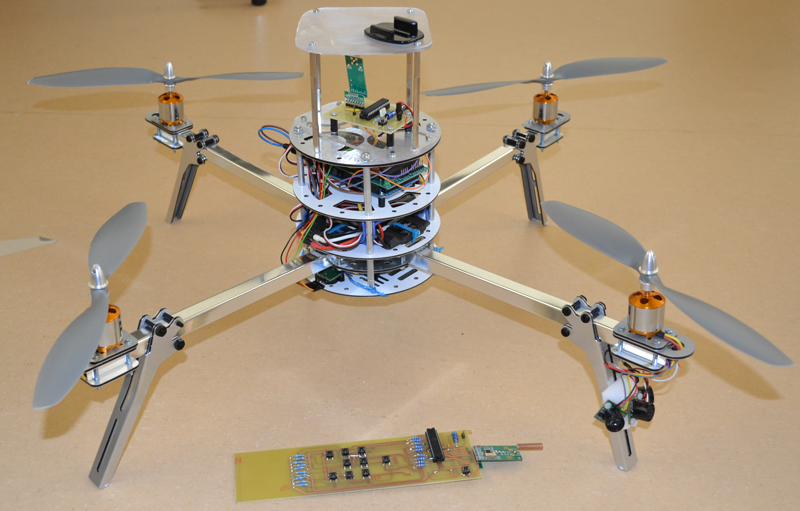
\includegraphics[width = \textwidth]{Billed}
\caption{Dronen og udviklet fjernbetjening}
\label{Fig:Billed}
\end{figure}


Projektet bestod i at lave 433 MHz trådløs styring af en drone.
Systemet skulle bestå af en fjernbetjening og en drone af type Cyclone fra firmaet AeroQuad\cite{AQ-store}. 
På figur \ref{Fig:Billed} ses et oversigt over det samlede system. 
Målet var at kunne styre dronen med en fjernbetjening, ved en frekvens på 433 MHz. 
Derudover skulle dronen også være i stand til at holde sin højde konstant. 
Dronen skulle også selv kunne undgå at flyve ind i objekter foran den, selvom brugeren beder den om det.

Systemet består af:
\vspace{-10pt}
\begin{enumerate}
\item AeroQuad-dronen Cyclone
\item En trådløs fjernbetjening
\end{enumerate}



\end{document}